%!TEX root = main.tex


\section{Implementation and Usage}

With explicit managed state and consistent snapshotting at its core, Flink maintains a rich ecosystem of backends, connectors and other services that interplay seamlessly and benefit from Flink's core mechanism. In this section, we summarize how most of these subsystems build on-top of Flink's core architecture, while expanding it with asynchronous communication, delivery guarantees and external state querying support.

\label{sec:implementation}

\subsection{State Backend Support}

Managed state consistency is coordinated by Flink's snapshotting algorithm (\autoref{sec:snapshots}), however, it is the responsibility of the state backends to handle state access and snapshotting for their respective state partitions. We distinguish two main classes of state backends: 1) \emph{Local State Backends}, where access to state is kept and controlled in the same physical node, and 2) \emph{External State Backends}, where state access is internally coordinated with an external system such as a database or key/value store.

\para{Local state}
 backends maintain all state in local memory or out-of-core, within an embedded key-value database such as RocksDB \cite{CUSTOM:web/rocksdb}. Out-of-core access is preferred in production deployments as in that case state size is only limited by the quota of the local file system allocated to each node. When a snapshot operation is triggered, a copy of the current local states is written to a durable storage layer (e.g. a distributed file system directory). The local state backends can support asynchronous and incremental snapshotting (\autoref{sec:async}) and yield considerable read/write performance as they exploit data locality while eliminating the need for distributed or transactional coordination.

\para{External state}
 backends coordinate state access with external database management systems. There are two possible variations, depending on the properties of the external database: 1) \textbf{Non-MVCC} (Multi-Version Concurrency Control) databases, can be supported by maintaining within each task a write-ahead-log (WAL) of pending state changes per epoch. The WAL can be committed to the database once an epoch has been completed. In more detail, each snapshot is one distributed bulk 2-phase commit transaction: during a checkpoint, changes are put into the transaction log (WAL) and pre-committed when \texttt{triggerSnapshot()} is invoked. Once the global snapshot is complete, the all pre-committed states are fully-committed by the JobManager in one atomic transaction. This approach is feasible even when the database does not expose the necessary program hooks to log, pre-commit, and fully commit.
 2) \textbf{MVCC-enabled} databases allow for committing state across multiple database versions. This can integrate with Flink's snapshotting mechanism by associating each state update with the undergoing epoch. Once a snapshot is fully committed the version is atomically incremented. Likewise, a failed snapshot epoch decrements the current version. A general advantage of external state backends is that rollback recovery does not require any I/O to retrieve and load state from snapshots (contrary to local state backends). This benefit becomes particularly impactful when state is very large, by avoiding any network I/O upon reconfiguration, thus, making it a suitable choice under strong latency requirements. Finally, another benefit that comes out-of-the-box with all external backends is support for incremental snapshotting, since, by definition, only changes are committed externally.
 
 %recovery compared to local states. Local state backends usually need to re-create their state mapping by reading the snapshot back before normal processing can start, whereas external backends can start processing immediately after the task was rescheduled on recovery 
 %In both cases the final commit is invoked centrally by the JobManager as an atomic transaction. Failures during the final commit can be eventually reconsiliated upon recovery by the Job Manager since both the WAL and the distributed MVCC transaction can be kept within the snapshot metadata and repeated.
 %State reads occur either locally (if they access uncommitted state), or more often, remotely in the database for committed state. 
 %The frequency of the epochs defines the size of the WAL. More frequently triggered snapshots 
 %after a successful within one checkpoint epoch as an atomic transaction%
%For the transactional approach n notifications of eventually completed checkpoints are received on each task. If the database supports MVCC, 


%\stephan{I honestly find the distinction between the In-Memory and File-based state backends confusing. Both hold working state in memory, and both write state to file systems on checkpoints (at least in HA mode) - the difference is to minor for a section in this paper. I also don't think that details about what state backends require additional serialization and which does not is relevant to conceptually understand the role of state backends and how the dataflow snapshots and the operator snapshots interact.}

%\stephan{Suggestion: We can go even broader here: I would describe that the responsibility of the state backend is to define the access to the state and how a snapshot of the state governed by the parallel task is taken. That gives us conceptually two types of state backends: (1) State backends that hold stat in-process in some map, and (2) state backends that interact with external databases or k/v stores. For (1) We have a state backend that uses hash maps (in memory) or RocksDB (out of core). For (2), we can again describe two implementations, (a) transactionally and (b) with MVCC (multi-version concurrency control). For (a) it works as follows: Each checkpoint is one distributed bulk 2-phase commit transaction: during a checkpoint, changes are put into the transaction log, on checkpoint they are pre-committed, and when the checkpoint as a whole is complete, the transaction is full-committed. The fact that practically most databases do not expose the fine grained hooks to log, pre-commit, and full commit can be worked around by maintaining an own write-ahead log and triggering bulk-load of the write-ahead log as a transaction upon completed checkpoints. (b) MVCC is simpler, the version of each change is that of the checkpoint epoch, and a commit bumps the version, while a failed checkpoint drops the current version (its harder in practice, because again most MVCC databases lack the hooks, but its a nice way to think about the problem).
%Let me know what you think! There is a bit of overlap with the "Consistent Output Commit" section.}

%\para{File-Based:}
%Most often, complete snapshots involve more aggregated state than the allocated memory of a single node. The \emph{File-Based} backend deviates from \emph{In-memory} only when it comes to snapshotting. Once a snapshot is invoked the state is being copied to a configured distributed file system directory (e.g., HDFS). As a result, snapshot metadata is also kept to a minimum, while throughput can remain high since operations on uncommitted state occur in-place at the local heap.

%\para{Out-of-Core:}
%Complex pipelines often need to maintain very large managed state such as long sliding windows. In such cases, local heap space is insufficient to sustain even locally accessed active state, especially for certain task operators (e.g., Flink's \texttt{WindowOperator}). Flink provides an \emph{out-of-core} backend that decouples state operations performed on each task from the physical location where state itself is persisted and updated. In its current implementation, out-of-core state is interfaced with an embedded file-backed key-value database (i.e., RocksDB). Therefore, state capacity is only limited by the file system space allocated at the host where this backend is deployed. Moreover, operations triggered on managed state such as \texttt{update} and \texttt{add} are carried over to the embedded key-value store instead. One of the key benefits, enabled out-of-the-box with such a scheme is that state updates can be executed asynchronously at the backend to maximize throughput. However, the main trade-off of accessing state off-heap is the extensive serialization overhead on each state access which can lead to lower throughput compared to heap-based active state. Nevertheless, this can be amortized, yielding less overhead during garbage collection (on-heap), flexible data locality, and copy-on-write support. An alternative version of the in-memory backend that operates on serialized data is currently considered to exploit the same benefits.

%\stefan{One big difference to the in-memory backends, and also a big source% of performance loss, is that this backend has to use serialization on each state read or update! Apart from this backend, keeping data serialized also has some advantages over objects on the heap: less overhead for the garbage collector, potentially higher data locality, and easier supoort for copy-on-write. This is why we are also planning to have an in-memory backend that works on serialized data.}. On the other hand, state value retrievals can take more time to complete, especially if some specific state has to be retrieved from compacted files on disk and it is no longer within the backend's memory.

\subsection{Asynchronous and Incremental Snapshots}
\label{sec:async}
One of the assets of the pipelined snapshotting protocol presented in \autoref{sec:snapshots} is that it does not inhibit the actual acquisition of snapshots to be synchronous. The \texttt{triggerSnapshot()} call by each task is expected to create an identical copy of the current state of that task. However, the copy is not required to be a physical copy, it can be a \emph{logical} snapshot that is \emph{lazily} materialized by a concurrent thread. This type of operation is supported by many \emph{copy-on-write} data structures. More concretely, Flink's local backends allow for asynchronous snapshots as such:

%One of the advantages of the pipelined snapshotting protocol presented in \autoref{sec:snapshots} is that it does not restrain the actual acquisition of snapshots to be synchronous. A call of \texttt{triggerSnapshot()} by each task is expected to create an identical copy of the current state of that task. In case there is support by a backend module to execute this operation asynchronously, it can be used without violating consistency.

The out-of-core state backend based on RocksDB \cite{CUSTOM:web/rocksdb} exploits the LSM (log-structured merge) tree, internal representation of data in RocksDB. 
%\footnote{\url{https://www.facebook.com/notes/facebook-engineering/under-the-hood-building-and-open-sourcing-rocksdb/10151822347683920/}}
Updates are not made in-place, but are appended and compacted asynchronously. Upon taking a snapshot, the synchronous \texttt{triggerSnapshot()} call simply marks the current version, which prevents all state as of that version to be overwritten during compactions. The operator can then continue processing and make modifications to the state. An asynchronous thread iterates over the marked version, materializes it to the snapshot store, and finally releases the snapshot so that future compactions can overwrite that state. Furthermore, the LSM-based data structure also lends itself to incremental snapshots, which write only parts to the snapshot store that changed since the previous snapshots.

Flink's in-memory local state backend implementation is based on an open-addressing hash table. During a snapshot, it copies the current table array synchronously and then starts the external materialization of the snapshot, in a background thread. The operator's regular stream processing thread lazily copies the state entries and overflow chains upon modification, if the materialization thread still holds onto the snapshot. Incremental snapshots for the in-memory local backend are  possible and conceptually trivial (using delta maps), yet not implemented at the current point. 

%The \emph{out-of-core} backend of Flink offers the capability to trigger snapshots in a purely asynchronous way by copying all key-value states belonging to the current snapshot to a backup directory concurrently by another thread, thus, letting normal processing proceed without interruptions. \TODO{In RocksDB, for example, this is done by iterating exclusively through the RocksDB snapshot created at the time of the checkpoint. }
%\stefan{Right now I am also working on an asynchronous in-memory state backend. For the future we are planning to also allow for incremental snapshots of the RocksDB backend. If you want more information about this, let me know.} 
%Once local snapshotting operations have been completed the notifications are triggered back at the tasks and carried out to the \emph{JobManager} alongside associated meta-data where a full snapshot is declared complete. 
%Asynchronous snapshotting also unlocks the possibility to have multiple instances of the protocol running at the same time in a dataflow graph. \gyula{I dont think asynch snapshots have much to do with this really.} That means that while for example a periodic snapshot is undergoing, a user can also trigger a savepoint and both of the associated snapshots will run concurrently and distributively, each invoking its own asynchronous state copy and epoch.

Finally, another feature that is provided to tasks as an optional asynchronous subscription-based mechanism is to trigger notifications about completed snapshots back at the tasks that request them. This is especially useful for garbage collection, discarding write ahead logs or for coordinating exactly-once delivery sinks as we explain further in \autoref{sec:outputcommit}.

\subsection{Queryable State}

A recent addition among Flink's state management features is the ability to directly query managed state from outside the system. External systems can access Flink's keyed-state in a similar way as that of a key/value store, providing read-only access to the latest values computed by the stream processor. This feature is motivated by two observations. First, it is required by many applications to grant ad-hoc access to the application state for faster insights. Secondly, eager publishing of state to external systems frequently becomes a bottleneck in the application as remote writes to the external systems cannot keep up with the performance of Flink's local state on high-throughput streams.

Queryable state allows for any declared managed state within a pipeline, currently scoped by key, to be accessed outside the system for asynchronous reading, through a subscription-based API. First, managed state that allows for query access is declared in the original application. Upon state declaration, introduced in \autoref{sec:managedstate}, it is possible to allow access from external queries by simply setting a flag in the descriptor that is used to create the actual state, having an assigned unique name for this specific state to be accessed, as such:

\begin{lstlisting}[language=scala]
//stream processing application logic
val descriptor: ValueStateDescriptor[MySchema] = ...
descriptor.setQueryable("myKV")
...
val mutState: ValueState[MySchema] = ctx.getState(descriptor)
\end{lstlisting}

\para{} Upon deployment, a state registry service gets initiated and runs concurrently with the task that holds write access to that state. A client that wishes to read the state for a specific key can, at any time submit an asynchronous query (obtaining a \texttt{future}) to that service, specifying the job id, registered state name and key, as shown below:

\begin{lstlisting}[language=scala]
//client logic
val client = QueryableStateClient(cfg);
var readState: Future[_] = client.getKVState(job, "myKV", key);
\end{lstlisting}
%MyDeserializer[MySchema](Await.result(readState, timeout));

The current implementation of queryable state supports point lookups of values by key. The query client asks the Flink master (JobManager) for the location of the operator instance holding the state partition for the queried key. The client then sends a request to the respective TaskManager, which retrieves the value that is currently held for that key from the state backend. From a traditional database isolation-level viewpoint, the queries access \emph{uncommitted state}, thus following the \emph{read-uncommitted} isolation level. As future work, we plan to add \emph{read-committed} semantics by letting TaskManagers hold onto the state of committed snapshots, and use that state to answer  adhoc queries.

%compared to already provided \emph{read-committed} read isolation guaranteed by its specialized sinks through its snapshotting mechanism (see \autoref{sec:outputcommit}).

\subsection{Exactly-Once Delivery Sinks}
\label{sec:outputcommit}

%\stephan{How about 'Exactly-once sinks'?}

%\stephan{I would suggest to also change this section to follow a more conceptual view. There are two types of sinks (1) Transactional sinks and (2) idempotent sinks (and (2.1) exactly-once state can turn non-idempotent sinks into idempotent sinks).}

So far we have considered consistency guarantees associated with the internal state of the system. However, it is most often important to offer guarantees regarding the side effects that a pipeline leaves to the outside world, whether that is a distributed database, file system or message queue. A pipeline interfaces with the outside world mainly via its dataflow sinks. Therefore, it is crucial that sinks can offer exactly-once delivery guarantees. The feasibility of achieving ``read-committed'' isolation guarantees to external writes depends on the properties of the system upon which sinks commit output and typically comes at a higher latency cost (this can, at-times, violate strong SLAs on latency). A pipeline can always be halted between snapshots after a failure or an urgent reconfiguration request and both input and state can be rolled back consistently, as it was described in \autoref{sec:core}. However, the same cannot always be guaranteed about the output. If sinks are connected, for example, to a printer that instantly flushes data on paper, a rollback would possibly print the same or alternating text twice. Flink's programming model is equipped with two main types of sinks that facilitate ``read-committed'' output and build on the snapshotting mechanism: 1) Idempotent and 2) Transactional Sinks.


%\stephan{For idempotent sinks: When a sink operation is truly \emph{idempotent}, no need to do anything (by definition). As an optimization, to avoid "read uncommitted", one can write changes to a write-ahead log and publish only when the checkpoint is completed (which makes it actually a transactional sink). When updates by key are not idempotent, one can make them idempotent by having a copy of the state in Flink's managed state, apply the changes to the Flink-managed state (which is exactly once) and pushing out the new values from that state (either directly or on checkpoint complete).}

\para{Idempotent Sinks: } Idempotency is a property used extensively by many systems at the presence of failures in order to encourage repeatability and alleviate bookkeeping efforts and complex transactions to offer delivery guarantees\cite{CUSTOM:web/SparkStructuredStreaming,millwheel}. In some cases deterministic pipeline logic and idempotency can already be offered by the stream application (e.g., not involving stream interleaving or other forms of non-determinism). For those cases, sinks need to take no further actions to achieve exactly-once delivery guarantees than eagerly publishing their output. However, if the end-to-end application logic cannot tolerate uncommitted reads a write-ahead-log (WAL) needs to be coordinated with asynchronous snapshot notifications to publish changes to the external system when an epoch has been completed. Flink's Cassandra database sink maintains a WAL of prepared query statements as part of its state. Once an asynchronous notification (\autoref{sec:async}) arrives for an epoch, the database sink commits all pending writes to the database. Query idempotency guarantees that even failures during publishing changes can be resolved by simply re-committing the same queries and thus, eventually, leaving the same side effects upon subsequent system reconfigurations. 

%\stephan{The transactional sinks come in two flavors: (1) Works like 2-phase commit: on shapshot (= pre-commit) they ensure persistence of their data and on "notify checkpoint complete" they commit. Example of that variant is a transactional SQL sink (possibly realized with a Flink-managed write-ahead-log), or any write-ahead-ligging sink. Sub-flavor (2) is always writing and rolling back on failures, exemplified by the rolling file sink. On snapshot (= pre-commit) ensures persistence (flush / sync to filesystem) and remember their version, on failure rollback (truncate file)}

\para{Transactional Sinks: } When idempotency cannot be guaranteed, committing output to external systems (e.g., File Systems, DBMSs) has to be made in a coordinated, transactional way. We identify two variants of this approach:

1) Maintaining a WAL at the sinks and eventually publishing it when a snapshot notification arrives locally using a 2-phase commit with the external system. An example of this approach is Flink's transactional SQL sink which includes in the sink's state the WAL to be committed. Eventually all changes are committed across partitions at the first successful snapshot. 

2) Alternatively, another approach that works well in conjunction with distributed file systems is to append uncommited output eagerly by every sink. On snapshot, output partitions can be pre-committed (e.g., by flagging a file directory) and eventually committed once the global snapshotting process is complete and notified across partitions. Upon failure changes can be rolled back. An example of this approach is Flink's \emph{bucketing} file sink (depicted in \autoref{fig:filecommit}) which eagerly appends stream output within uncommitted distributed file directories which group (or ``bucket'') file partitions by time-period. After a pre-configured inactivity time-period \texttt{in-progress} directories become \texttt{pending} and are ready to be committed. The Bucketing File Sink integrates with Flink's snapshotting algorithm and associates epochs with buckets. Once a file bucket is under \texttt{pending} mode and an asynchronous notification for an associated epoch has been received, it can be moved to a \texttt{committed} state via an atomic \texttt{rename} operation. Potential disruptions between epochs resolve into a \texttt{truncate} (Posix) operation, which is currently supported by major distributed file systems and conveniently reverses append operations to the right epoch.


\begin{figure}[t!]
\centering
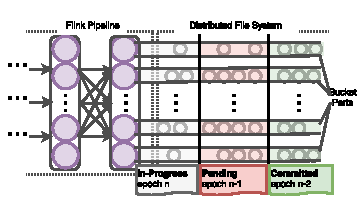
\includegraphics[width=\textwidth / 2]{figures/filecommit.pdf}
\caption{A visualization of Bucketing File Sinks.} 
\label{fig:filecommit}
\vspace{-2mm}
\end{figure}


%\subsection{Asynchronous IO}
%\paris{What I write here does not seem to be the actual implementation. The implementation does event sourcing which is a bit sucky tbh...}
%Most often, all logic within a pipeline is executed within its stateful tasks and data ingestion from external systems flows directly through pipeline sources. Flink enforces this restriction in order to guarantee consistent, managed state and more importantly to avoid \emph{blocking} operations that can create a bottleneck or even a deadlock in a pipeline. If the application logic deems access to external systems necessary, Flink offers an Asynchronous I/O model for such operations. 

%Special \texttt{AsyncIO} operators in Flink, provide the necessary callbacks for invoking and handling asynchronous, user-defined requests to external systems (e.g., a database). Asynchronous requests are internally logged and maintained as part of the managed state of \texttt{AsyncIO} operators. Responses are also logged in-advance as part of the state and their handling can be optionally pre-configured to be FIFO according to their invocation or event time order (based on low watermarks \cite{millwheel,akidau2015dataflow,li2008out}). Asynchronous operations integrate seamlessly with the core snapshotting algorithm since both invocation and handling logic is executed within the same regular processing thread of the encapsulating task, thus, yielding atomic and controlled access to managed state. In case of rollback recovery, all logged requests are being repeated and pending results are eventually processed within their respective epoch in the pre-defined order. There are no guarantees, whatsoever, regarding the side effects of potential async write operations that will be repeated in case or rollback recovery on external systems. Similarly to Google's Millwheel \cite{millwheel},  all async I/O operations that communicate with external systems should be idempotent to satisfy strong consistency guarantees on those systems.

\subsection{High Availability \& Reconfiguration}

All metadata associated with the active state of long-running pipelines is kept within the \texttt{JobManager} node. This makes the importance of this central node quite high for the general functionality of the system but also a single-point-of-failure. A \texttt{JobManager} failure would halt the coordination of the snapshotting protocol, the collection and management of snapshot metadata as well as making further job deployments and rescaling requests unavailable, thus, eliminating the purpose of any fault tolerance mechanism. To deal with such a critical failure we employ a passive-standby high availability scheme where configured standby nodes can take undertake the coordination role of the failed master node via distributed leader election. When this mode is enabled, the coordination of vital decisions such as job deployment and scheduling are undertaken via a distributed decision protocol which logs committed operations atomically (currently utilizing a \texttt{Zookeeper} quorum executing the \texttt{zab} protocol \cite{hunt2010zookeeper}). This introduces some additional latency for such critical operations, however, non-critical decisions such as the persistence of the most recent snapshot metadata for a job, are asynchronously committed and logged. The worst scenario of a potential failure during non-critical commits would simply result into, a yet valid restoration of active pipeline state from consistent snapshots that correspond to earlier epochs that have been committed prior to the failure.

	